%
% Complete documentation on the extended LaTeX markup used for Insight
% documentation is available in ``Documenting Insight'', which is part
% of the standard documentation for Insight.  It may be found online
% at:
%
%     http://www.itk.org/

\documentclass{InsightArticle}


%%%%%%%%%%%%%%%%%%%%%%%%%%%%%%%%%%%%%%%%%%%%%%%%%%%%%%%%%%%%%%%%%%
%
%  hyperref should be the last package to be loaded.
%
%%%%%%%%%%%%%%%%%%%%%%%%%%%%%%%%%%%%%%%%%%%%%%%%%%%%%%%%%%%%%%%%%%
\usepackage[dvips,
bookmarks,
bookmarksopen,
backref,
colorlinks,linkcolor={blue},citecolor={blue},urlcolor={blue},
]{hyperref}
% to be able to use options in graphics
\usepackage{graphicx}
% for pseudo code
\usepackage{listings}
% subfigures
\usepackage{subfigure}


%  This is a template for Papers to the Insight Journal. 
%  It is comparable to a technical report format.

% The title should be descriptive enough for people to be able to find
% the relevant document. 
\title{Morphology with parabolic structuring elements}

% Increment the release number whenever significant changes are made.
% The author and/or editor can define 'significant' however they like.
\release{0.00}

% At minimum, give your name and an email address.  You can include a
% snail-mail address if you like.
\author{Richard Beare}
\authoraddress{Richard.Beare@monash.edu\\Department of Medicine\\Monash University\\Melbourne\\Australia}

\begin{document}
\maketitle

\ifhtml
\chapter*{Front Matter\label{front}}
\fi


\begin{abstract}
\noindent
It is often useful to be able to compute the component of image
gradient in a direction defined by a shape of some form, rather than
relative to the image axis. This article introduces a simple method
for doing this based on distance transforms that is potentially useful
in a number of applications.
\end{abstract}

\tableofcontents

\section{Introduction}
The gradient of a greyscale image is a vector pointing in the
direction of maximum rate of change on intensity. It is often
desirable to compute the component of this gradient relative to
directions derived from image data, such as a mask representing domain
knowledge. One simple and useful way of doing this is implemented in
the {\em itkDirectionalGradientImageFilter}, introduced in this
article.

\section{Algorithm}
Prior knowledge is represented by a mask, with direction being
computed relative to the edges of the mask. This is achieved by
computing the gradient of the distance transform of the mask, which
provides a simple way of computing directions at positions away from
the mask edges. The component of the gradient parallel to this
direction can then be computed using an inner product.

\section{Applications and Examples}
The directional gradient can be useful in a number of situations, such
as distinguishing interior and exterior edges of walls or computing
gradients in the presence of clutter. Simple examples using the
cthead1 image are illustrated in Figres \ref{fig:source_and_mask} to
\ref {fig:dl}. The mask used in this example is a small region near
the middle of the image. The gradient of the distance transform of
this mask is therefore pointing directly away from this region, with
contours of the distance transform image forming circles around the
image centre. Note that this mask could be a sinlge voxel, but has
been enlarged for simpler visualization. This mask represents a very
simple form of prior knowledge - points known to be inside the
skull. Given this prior knowledge it is simple to separate light to
dark transitions from dark to light transitions as we travel away from
masked voxels. These images were generated using {\em testDirectional}
and {\em label\_overlay}, included with this package.

\begin{figure}[htbp]
\centering
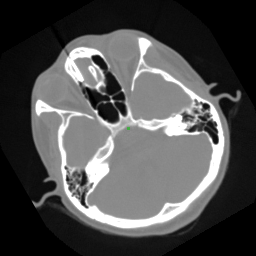
\includegraphics[scale=0.75]{source_and_mask_ov}
\caption{Raw image with mask representing prior knowledge (overlaid in green).\label{fig:source_and_mask}}
\end{figure}

\begin{figure}[htbp]
\centering
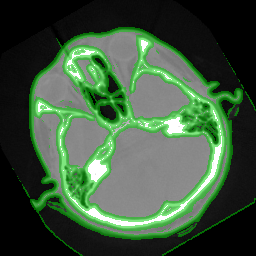
\includegraphics[scale=0.75]{grad_ov}
\caption{Standard linear gradient (thresholded).\label{fig:grad}}
\end{figure}

\begin{figure}[htbp]
\centering
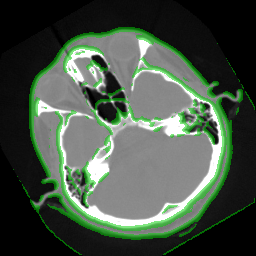
\includegraphics[scale=0.75]{light_to_dark_ov}
\caption{Light to dark transitions (thresholded).\label{fig:ld}}
\end{figure}

\begin{figure}[htbp]
\centering
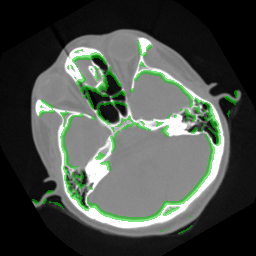
\includegraphics[scale=0.75]{dark_to_light_ov}
\caption{Dark to light transitions (thresholded).\label{fig:dl}}
\end{figure}

\section{Usage}
This algorithm is implemented in the {\em
  itkDirectionalGradientImageFilter} included with the article. It is
a simple mini-pipeline filter that utilizes standard ITK gradient
filters, a new inner product filter and the fast distance transform
filters from an earlier InsightJournal publication \cite{Beare2008e}. The filter has a simple interface with only 3 control parameters:
\begin{itemize}
\item {\em SetOutsideValue}: controls the behaviour of the distance transform. The default (0), implies computing the distance to the nearest voxel with value 0. This is set to 1 for the example.
\item {\em SetSigma}: controls the size of the smoothing kernel used in computation of the gradient of the raw image.
\item {\em SetScale}: controls a scaling factor using in the inner product. This is a convenient way of forcing the output gradient to always be positive. 
\end{itemize}
Complete usage is illustrated in {\em testDirectional.cxx}.

\section{Source code}
Source code is available in with this article and latest versions are
available from via git from
\url{https://richardbeare@github.com/richardbeare/DirectionalGradient.git}.
\section{Conclusion}
This is a simple filter implementing a trick that I have found useful
on a number of occasions. I hope the community finds it useful and/or
interesting too.

\bibliographystyle{plain} \bibliography{local,InsightJournal}
\nocite{ITKSoftwareGuide}

\end{document}

